\chapter{評価}
\label{chap:evaluation}

\ref{chap:network-transmission}章ての映像制作現場におけるIP伝送装置の要件に基づいて、ソフトウェア、ハードウェアそれぞれIP伝送装置の実装を行った。
本章ではアプローチが有効な手法であるか、それぞれの項目について評価する。

\section{概要}

\ref{chap:software-experimentation}章、\ref{chap:implementation}章

AAA

\section{トラフィック}

トラフィックを計測した

\subsection{計測手法}

ソフトウェア実装の場合はにおける受信PC、ハードウェア実装の場合はIP分配折り返しボードに接続されたデバッグ用のPCで受信バイト数、受信パケット数、破棄パケット数を計測した。
インターフェースの情報は/proc/net/devを監視し、rrdtoolを使い集計、グラフとして出力した。

\subsection{計測結果}

\begin{figure}[htbp]
  \begin{center}
    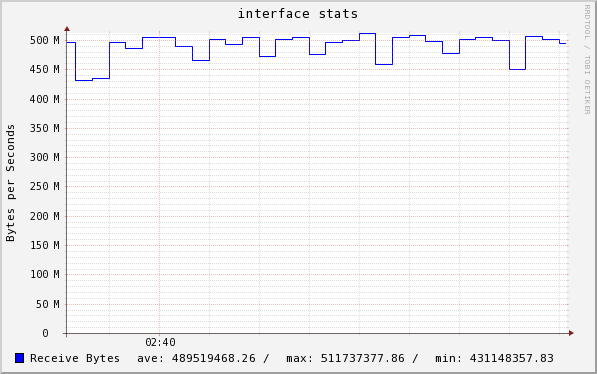
\includegraphics[bb=0 0 597 374,width=12cm]{img/lo-bytes-graph.png}
  \end{center}
  \caption{ソフトウェア実装における伝送中の受信バイトのグラフ}
  \label{fig:lo-bytes-graph}
\end{figure}

\begin{figure}[htbp]
  \begin{center}
    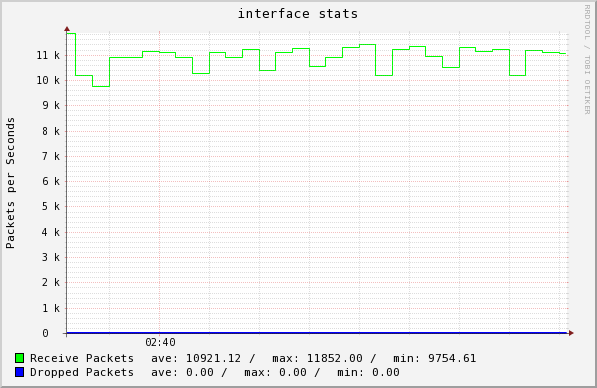
\includegraphics[bb=0 0 597 388,width=12cm]{img/lo-packets-graph.png}
  \end{center}
  \caption{ソフトウェア実装における伝送中の受信パケットのグラフ}
  \label{fig:lo-packets-graph}
\end{figure}

図\ref{fig:lo-bytes-graph}で示した、受信バイトのグラフでは平均489MBpsとなっている。
ソフトウェア実装での実データはYCbCr 4:2:2のピクセルあたり2bytesである。

3840 x 2160 x 2 * 30
フレームあたり

\begin{figure}[htbp]
  \begin{center}
    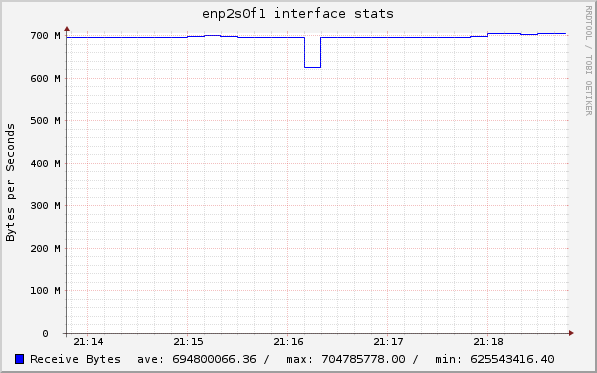
\includegraphics[bb=0 0 597 374,width=12cm]{img/enp2s0f1-bytes-graph.png}
  \end{center}
  \caption{ハードウェア実装における伝送中の受信バイトのグラフ}
  \label{fig:enp2s0f1-bytes-graph}
\end{figure}

\begin{figure}[htbp]
  \begin{center}
    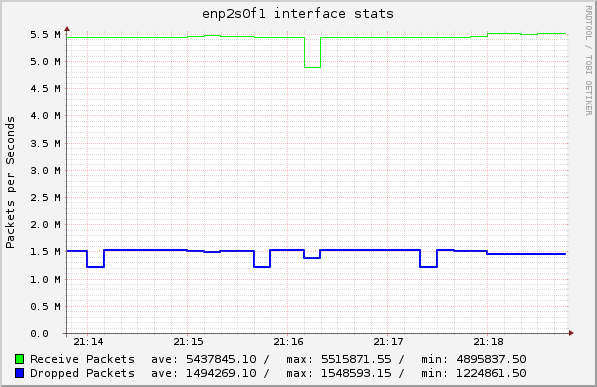
\includegraphics[bb=0 0 597 388,width=12cm]{img/enp2s0f1-packets-graph.png}
  \end{center}
  \caption{ハードウェア実装における伝送中の受信パケットのグラフ}
  \label{fig:enp2s0f1-packets-graph}
\end{figure}

% HDMIのデータとなるので、4:2:2でもRGBと帯域は変わらない
3840 * 2160 * 4 * 30=

694800066/5437845
平均127.77bytesのパケットとなる

190,924,575bytes

885,724,641bytesではないか

1-(14/127.77)=0.890
1-(56/127.77)=0.561

\newpage
\section{遅延}

遅延を計測した

\subsection{計測手法}

映像機器の遅延を計測するため、テスト信号生成、マルチビューワー生成、画面キャプチャーの機能を有する機器を用意した。
遅延を計測した機器の構成を図\ref{fig:evaluate-diagram}に示す。

テスト信号生成では、フレーム単位のタイムコードが表示された同じソースの映像を2つの信号として出力する。
一方をスイッチャーへ入力し、もう一方を検査対象となる機器に入力し、その出力をスイッチャーへ入力する。
これにより、2つの信号の遅延は、検査対象となる機器で発生した遅延に抑えることができる。
スイッチャーに入力された2つの信号はマルチビューワーとして1つの画面に表示され、その画面をキャプチャーすることにより、ある瞬間の2つの信号を1つの画像で確認することができる。
このスイッチャーには、フレーム同期の機能があり、1フレームより短い期間でバッファリングされるため、計測できる粒度はフレーム単位となる。

\begin{figure}[htbp]
  \begin{center}
    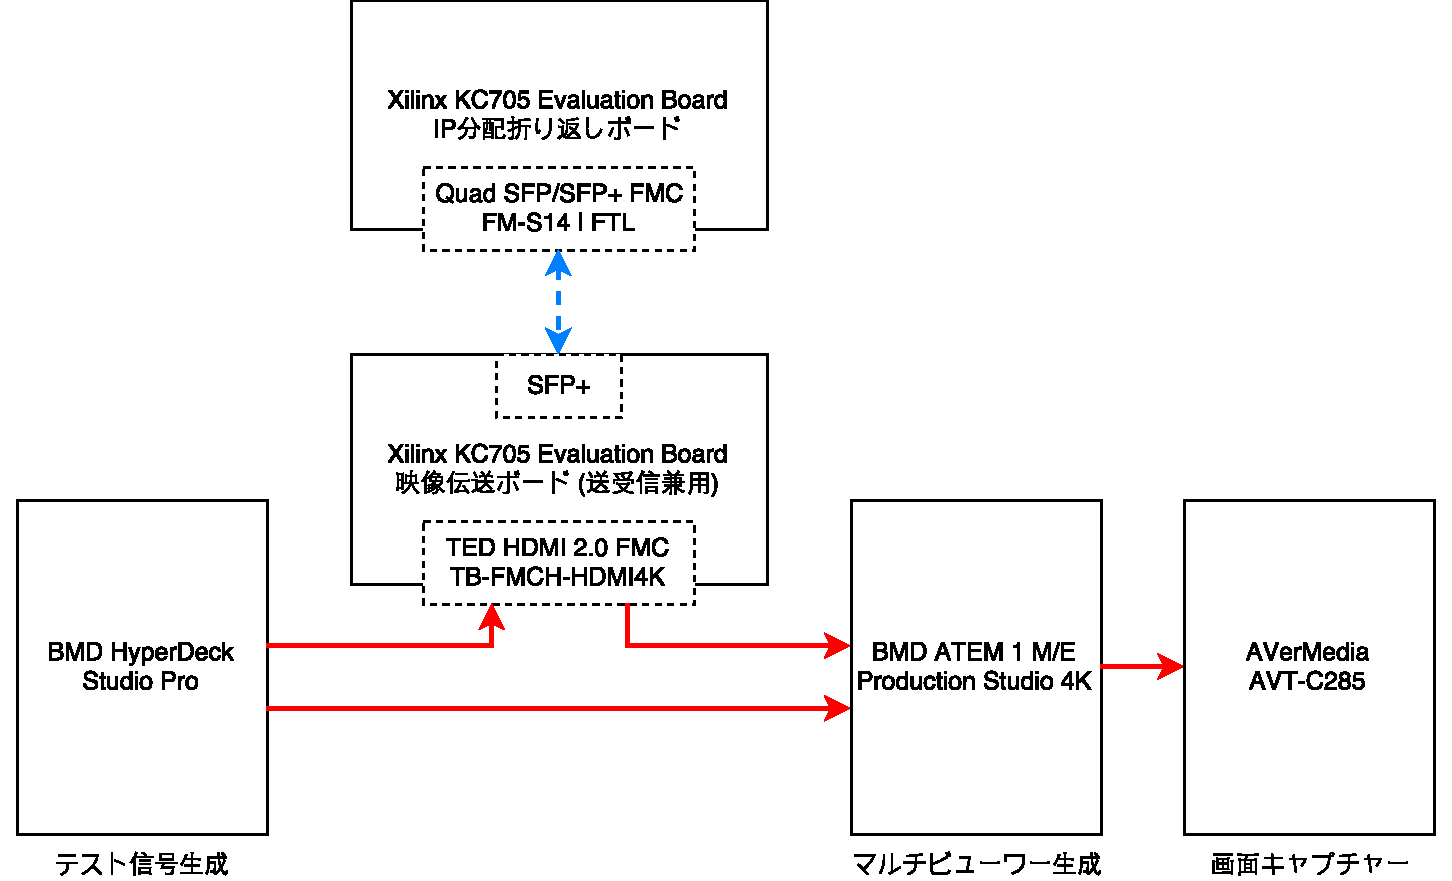
\includegraphics[bb=0 0 697 212,width=15cm]{img/evaluate-diagram.pdf}
  \end{center}
  \caption{遅延の計測手法}
  \label{fig:evaluate-diagram}
\end{figure}

\subsection{計測結果}

aaa

\begin{figure}[htbp]
  \begin{center}
    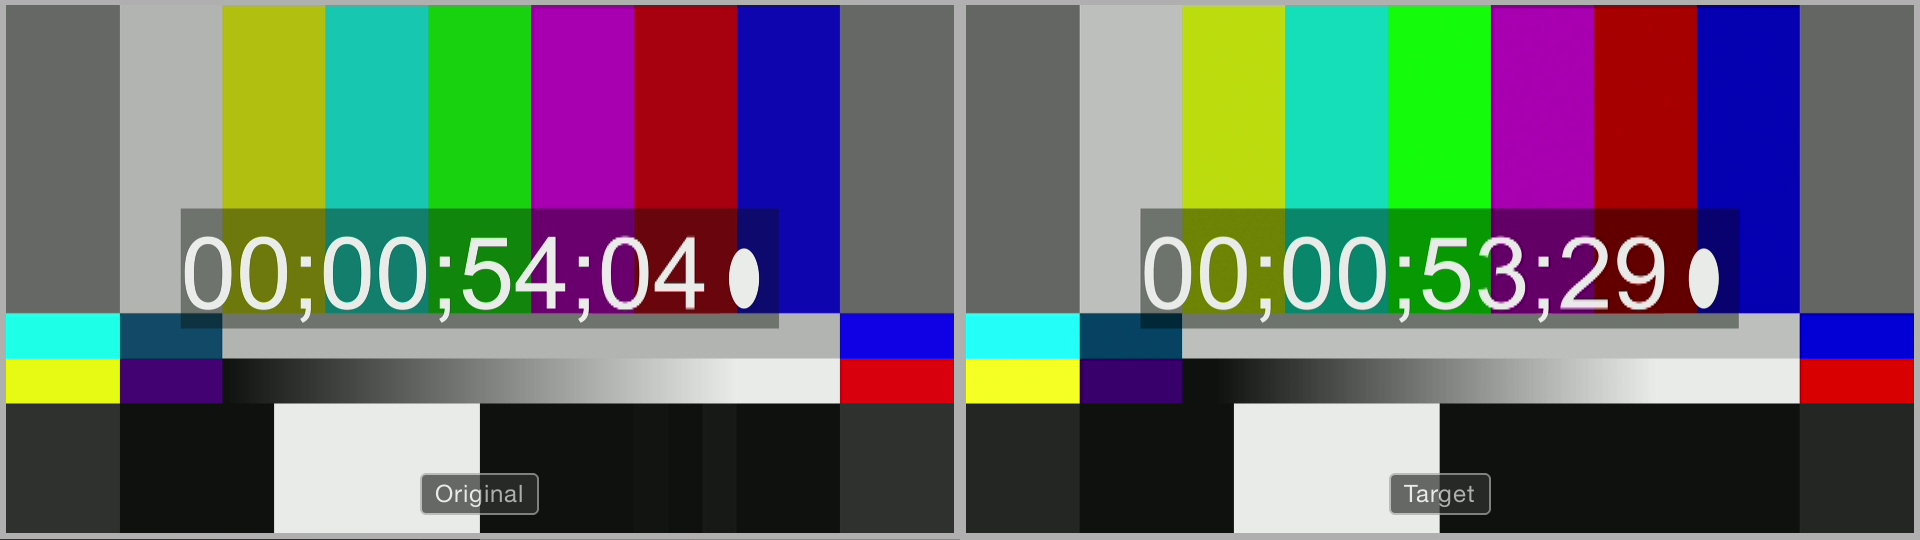
\includegraphics[bb=0 0 1920 540,width=14cm]{img/evaluate-delay-software-1.png}
  \end{center}
  \caption[ソフトウェア実装による遅延計測のキャプチャー画像]{ソフトウェア実装による遅延計測のキャプチャー画像 左がオリジナルの信号、右が検査対象の信号}
  \label{fig:evaluate-delay-software-1}
\end{figure}

\begin{figure}[htbp]
  \begin{center}
    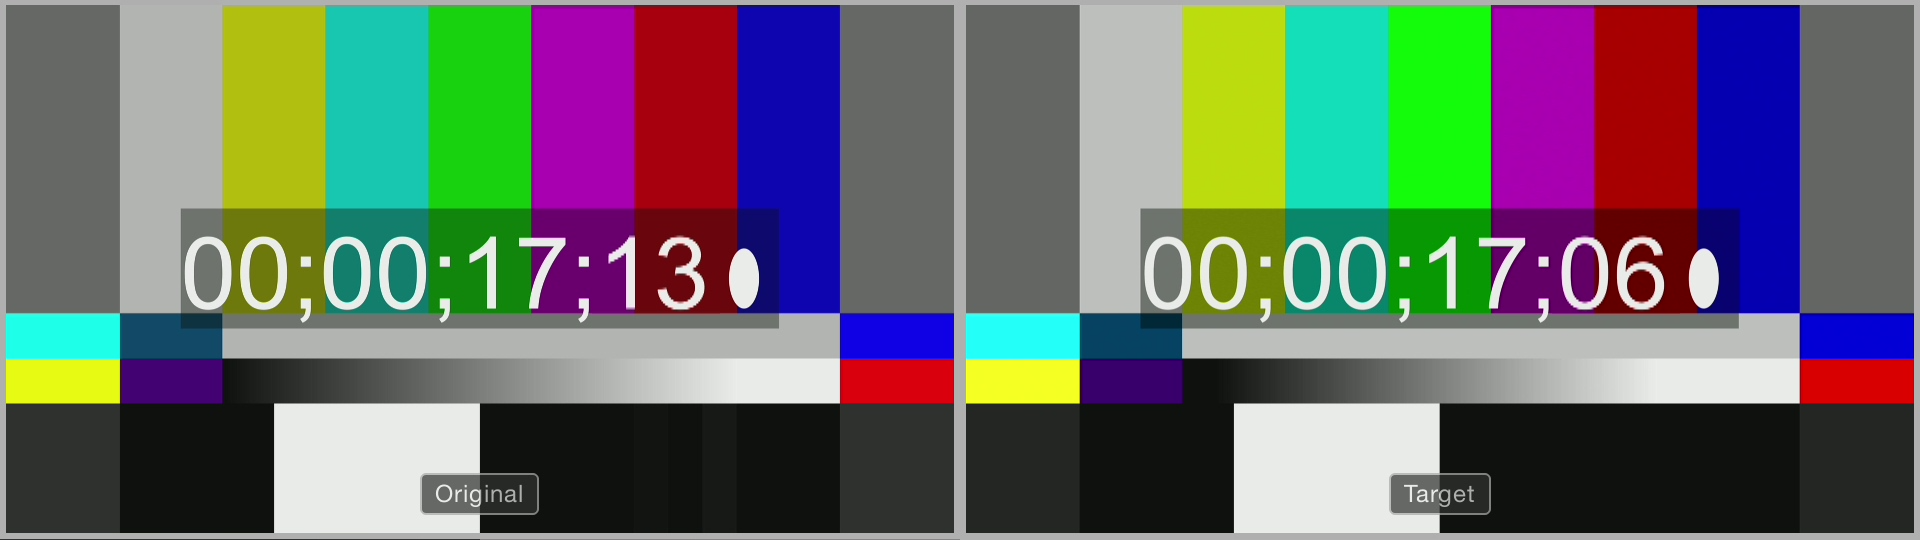
\includegraphics[bb=0 0 1920 540,width=14cm]{img/evaluate-delay-software-2.png}
  \end{center}
  \caption[ソフトウェア実装による遅延計測のキャプチャー画像]{ソフトウェア実装による遅延計測のキャプチャー画像 左がオリジナルの信号、右が検査対象の信号}
  \label{fig:evaluate-delay-software-2}
\end{figure}

\begin{figure}[htbp]
  \begin{center}
    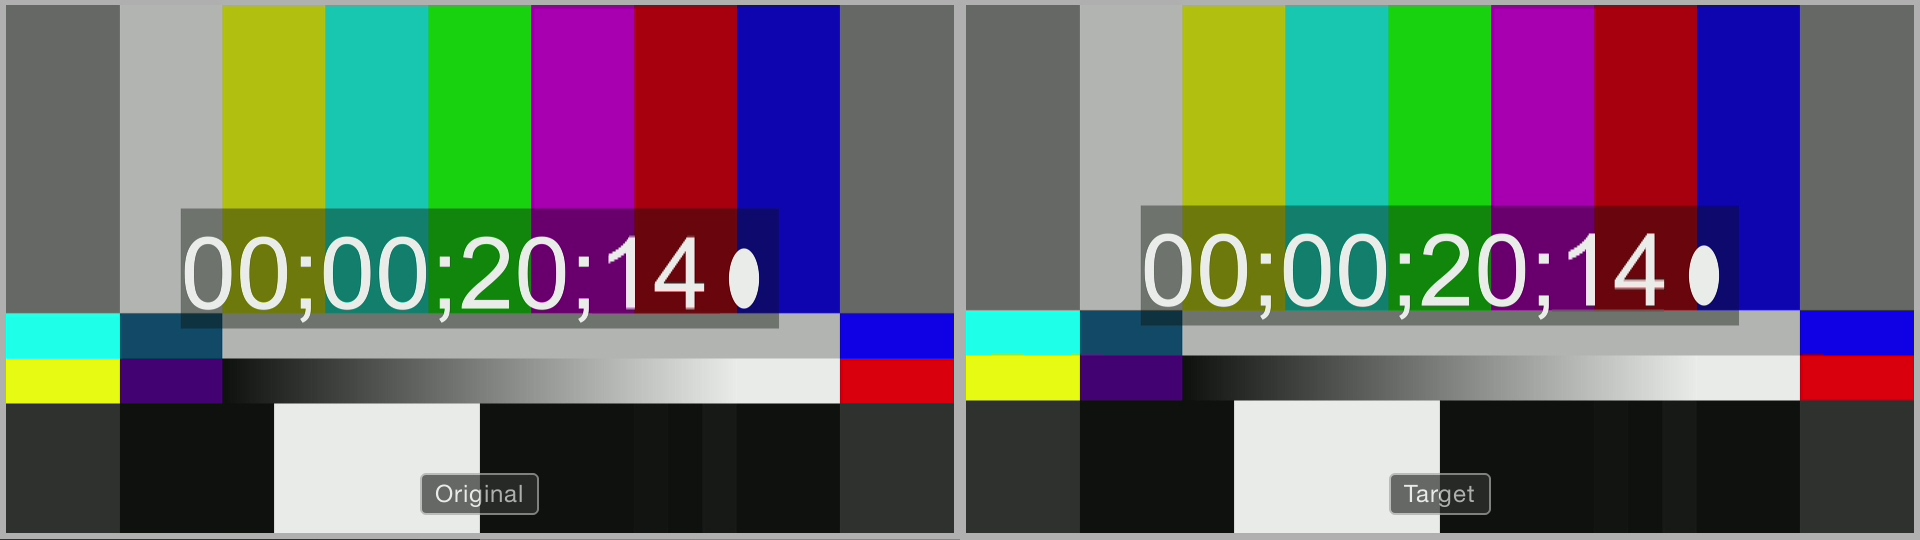
\includegraphics[bb=0 0 1920 540,width=14cm]{img/evaluate-delay-hardware.png}
  \end{center}
  \caption[ハードウェア実装による遅延計測のキャプチャー画像]{ハードウェア実装による遅延計測のキャプチャー画像 左がオリジナルの信号、右が検査対象の信号}
  \label{fig:evaluate-delay-hardware}
\end{figure}

\section{YCbCr 4:2:0}
あああ


% \begin{table}[htbp]
%   \caption{ソフトウェア実装による30FPSにおける遅延時間}
%   \label{tb:pg235-vin-axi4-stream}
%   \begin{center}
%   \begin{tabular}{l|c|c}
%     \hline
%          & 遅延時間  & 遅延フレーム \\\hline\hline
%     1回目 & 300 ms  & 9 frames \\\hline
%     1回目 & 300 ms  & 9 frames \\\hline
%     1回目 & 300 ms  & 9 frames \\\hline
%     1回目 & 300 ms  & 9 frames \\\hline
%     1回目 & 300 ms  & 9 frames \\\hline
%     1回目 & 300 ms  & 9 frames \\\hline
%     1回目 & 300 ms  & 9 frames \\\hline
%     1回目 & 300 ms  & 9 frames \\\hline
%     1回目 & 300 ms  & 9 frames \\\hline
%     1回目 & 300 ms  & 9 frames \\\hline
%     1回目 & 300 ms  & 9 frames \\\hline
%     1回目 & 300 ms  & 9 frames \\\hline
%     1回目 & 300 ms  & 9 frames \\\hline
%     1回目 & 300 ms  & 9 frames \\\hline\hline
%     平均  & 300 ms  & 9 frames \\\hline
%   \end{tabular}\end{center}
% \end{table}

\section{実証実験}
本実装に実用性があることを顕彰するため、ORF2015とORF2016でそれぞれ実証実験を行った。
付録\ref{chap:orf2015}、付録\ref{chap:orf2016}

\section{考察}
